%----------------------------------------------------------------
% FEUILLE DE STYLE ENSG au format Latex
% Création : sept. 2010 (D Lercier)
% Modification sept. 2012 (T Coupin)
%----------------------------------------------------------------

\documentclass{themeensg}
\usepackage[utf8]{inputenc}
\usepackage[T1]{fontenc}
\usepackage{lmodern} % load a font with all the characters
\usepackage{caption}
\usepackage{fancyhdr}
\usepackage{lastpage}
\usepackage[inline]{enumitem} % horizontal enumerations
\usepackage{tikz-uml} % UML
\usepackage{algpseudocode} % pseudo code
\usepackage{listings} % source code
 
\pagestyle{fancy}
\fancyhf{}
 
\rfoot{Page \thepage \hspace{1pt} of \pageref{LastPage}}

%---Texte en filigranne---
\SetWatermarkText{}
%pour l'enlever : \SetWatermarkText{}
%-------------------------

%---Mes packages à moi---
\usepackage[english, frenchb]{babel}
%------------------------

%---Mes raccourcis---
\newcommand{\transpose}[1]{{}^t \! #1}
\newcommand{\ensg}{\textsc{Ensg}}
%--------------------

%---Paramètres du pdf---
\hypersetup{
       backref=true,                           % Permet d'ajouter des liens dans
       pagebackref=true,                       % les bibliographies
       hyperindex=true,                        % Ajoute des liens dans les index.
       colorlinks=true,  %Colorise les liens : true pour version numérique, false pour version d'impression
       breaklinks=true,                        % Permet le retour à la ligne dans les liens trop longs.
       urlcolor= blue,                         % Couleur des hyperliens.
       linkcolor= blue,                       % Couleur des liens internes.
       bookmarks=true,                         % Créé des signets pour Acrobat.
       %bookmarksopen=true,                    % Si les signets Acrobat sont créés,
                                               % les afficher complètement.
       pdftitle={Clément Drouadaine Internship Report},               % Titre du document.
                                               % Informations apparaissant dans
       pdfauthor={Clément Drouadaine},                      % dans les informations du document
       pdfsubject={Internship report}           % sous Acrobat.
    }

%-----------------------



%-------------------------------------------------------------

\setcounter{tocdepth}{4} %profondeur de la table des matières
\setcounter{secnumdepth}{4}

\title{Developing a graphical user interface for the real-time ionosphere scintillation monitor}

%
%-------------------------------------------------------------
% Début du document
%--------------------------------------------------------------
\newlength\longest
\begin{document}
%--------------------------------------------------------------
\begin{titlepage}
%Inclusion des labels des entreprises
%Pour un seul label (à gauche), mettre NULL pour les 3e et 4e argument
%\enterprise 
\begin{minipage}{.5\textwidth}
  
\includegraphics[width=.5\linewidth]{images/logos/ensg_logo.png}
\end{minipage}
\begin{minipage}{.5\textwidth}
  \centering
  
\includegraphics[width=.5\linewidth]{images/logos/kartverket_logo.png}
\end{minipage}

%Prevents LaTeX from messing with spacing before and after colons
\shorthandoff{:}

%Inclusion du titre
\maketitle{Internship report \\ Cycle: 3\up{rd} year of engineering, GTSI specialization}
{Aurora_Borealis_Norway.jpg}

\infos{Clément Drouadaine}{September 2015}
\end{titlepage}


%---Page du jury---
%---Page du jury---
\newevenpage
\thispagestyle{plain}
\section*{Jury}
%Prevents LaTeX from messing with spacing before and after colons
\shorthandoff{:}

\vspace{0.5cm}

\textbf{President of jury:} \\

Pierre-Yves HARDOUIN

\vspace{0.5cm}

\textbf{Host Company:} \\

Kartverket

\vspace{0.5cm}

\textbf{Internship training supervisor:} \\ 

Oddgeir KRISTIANSEN \par
Emmanuel BARDIÈRE, ENSG \par
Vincent DE OLIVEIRA, ENSG

\vspace{0.5cm}

\textbf{Educational person in charge of the engineering course:} \\

Serge BOTTON, IGN/ENSG/DE/DPTS

\vspace{0.5cm}

\textbf{School's professional training counsellor:} \\

Patricia PARISI, IGN/ENSG/DE/DSHEI

\vspace{1cm}

\copyright \hspace{0.3cm} ENSG

\section*{Internship from 05/05/2015 to 25/09/2015}
\vspace{0.3cm}
\textbf{Web diffusion:} $\boxtimes$ Internet \hspace{0.2cm} $\boxtimes$ Intranet ENSG

\vspace{0.3cm}
\textbf{Document situation:} 

\vspace{0.2cm}
\par
Internship report presented in the end of the 3\up{rd} year of engineer cycle

\vspace{0.3cm}
\newcounter{x}
\setcounter{x}{\getpagerefnumber{LastPage}-\getpagerefnumber{beginappendices}+1}
\textbf{Number of pages:} \getpagerefnumber{LastPage} pages including \arabic{x} annexes

\vspace{0.3cm}
\textbf{Host system:} \LaTeX
\vspace{1cm}
%------------------


\clearpage

\thispagestyle{empty}
\null\vfill

\settowidth\longest{\huge\itshape It's still magic even if you know;}
\begin{center}
\parbox{\longest}{
  \raggedright{\huge\itshape
  It's still magic even if you know how it's done.\par\bigskip
  }
  \raggedleft\Large\underline{A Hat Full of Sky}\MakeUppercase{, Terry Pratchett}\par%
}
\end{center}
\vfill\vfill

\clearpage

%------------------------------------------------------------------------------
% Remerciements
\selectlanguage{english}
\newevenpage
\chapter*{Acknowledgements}

I would like to thank my internship supervisor in Kartverket, Rune Hanssen, for all the help and support he provided me all along the internship, and his availability whenever I needed him.

Thanks also to the whole of the geodesy department team for their welcome and especially Yngvild Linnea Andalsvik for her help, and Geir Arne Hjelle for the non work-related times we had.

Last but not least, I would like to give a big thanks to Zuheir Altamimi to whom I resorted once more to find me this internship. Like last year, I contacted him after unfruitful researches on my own, and he managed to find me an internship where I wanted, in the field I wanted, and within 24 hours. Once more, thank you very much.

%---Résumé (français)---
\selectlanguage{frenchb}
\begin{abstract}
\thispagestyle{empty}
	\vspace{1cm}

	
	
	\vspace{1.5cm}
	
	\textbf{Mots clés :} interface, web.
\end{abstract}
%-----------------------


%---Résumé (anglais)---
\selectlanguage{english}
\begin{abstract}
\thispagestyle{empty}
	\vspace{1cm}
	
	
	\vspace{1.5cm}
	
	\textbf{Key words:} interface, web, 
\end{abstract}
%----------------------



%---Table des matières, des figures et des tableaux---
\newevenpage
\tableofcontents

\newevenpage
\listoffigures

\newevenpage
\listoftables
%----------------------------------------------------

\newevenpage
\chapter*{Glossary and useful acronyms}
\addcontentsline{toc}{chapter}{Glossary and useful acronyms}

\begin{acronym}
  \acro{API}{Application Programming Interface}
  \acro{CPU}{Central Processing Unit}
  \acro{DE}{Direction de l'Enseignement = Education Department}
  \acro{DPTS}{Département du Positionnement Terrestre et Spatial = Terrestrial \& Spatial Positioning Department}  
  \acro{DSHEI}{Département des Sciences Humaines, des relations Entreprises et des relations Internationales = Social Sciences, Industry relations and International relations Department}
  \acro{ENSG}{École Nationale des Sciences Géographiques = National School of Geographic Sciences}
  \acro{ERR}{ERRor messages}
  \acro{GTSI}{Géomatique et Technologie des Systèmes d'Information = Geomatics and Technology of the Information Systems}
  \acro{GUI}{Graphical User Interface}
  \acro{IGN}{Institut Géographique National = National Geographical Institute}
  \acro{IP}{Internet Protocol}
  \acro{MON}{MONitoring table}
  \acro{OS}{Operating System}
  \acro{PHP}{PHP: Hypertext Preprocessor (recursive acronym)}
  \acro{PROC}{list of active PROCesses}
  \acro{RTIS}{Real-Time Ionosphere Scintillation monitor}
  \acro{SATREF}{SATellittbasert REFeransesystem = Satellite-based Reference System}
  \acro{SSH}{Secure SHell}
  \acro{TCP}{Transmission Control Protocol}
  \acro{UDP}{User Datagram Protocol}
  \acro{UML}{Unified Modelling Language}
\end{acronym}


%---Introduction------------------------------------------------------------------
\newevenpage
\chapter*{Introduction}
  \addcontentsline{toc}{chapter}{Introduction}
  
  \vspace{1.5cm}
	
%-------------------------------------------------------------------------------

\evenchapter[Definition of the objectives]{Definition of the objectives}

%-------------------------------------------------------------------------------
\section{What RTIS is: a brief overview}

TEXT HERE

All stations run a Ubuntu or Ubuntu-based operating system. Limit use of resources to not overwrite data in the meantime.

%-------------------------------------------------------------------------------

\section{What exists to monitor it: description of the existing}

Before my arrival at Karverket, there was only one way of monitoring a distant RTIS stations: connecting to it via SSH, and manually launch a monitoring program, called \textit{rtis\_mon}, on the console. Depending on the parameter it is given, this displays a table containing either information about the running processes (option \textit{-proc}), different values relevant to monitoring the performances of RTIS (option \textit{-mon}) or data about ephemeris (option \textit{-eph}). This \textit{rtis\_mon} program will then run indefinitely until it is stopped, and update its values approximately once every second.

\begin{figure}[!ht]
	\centering
	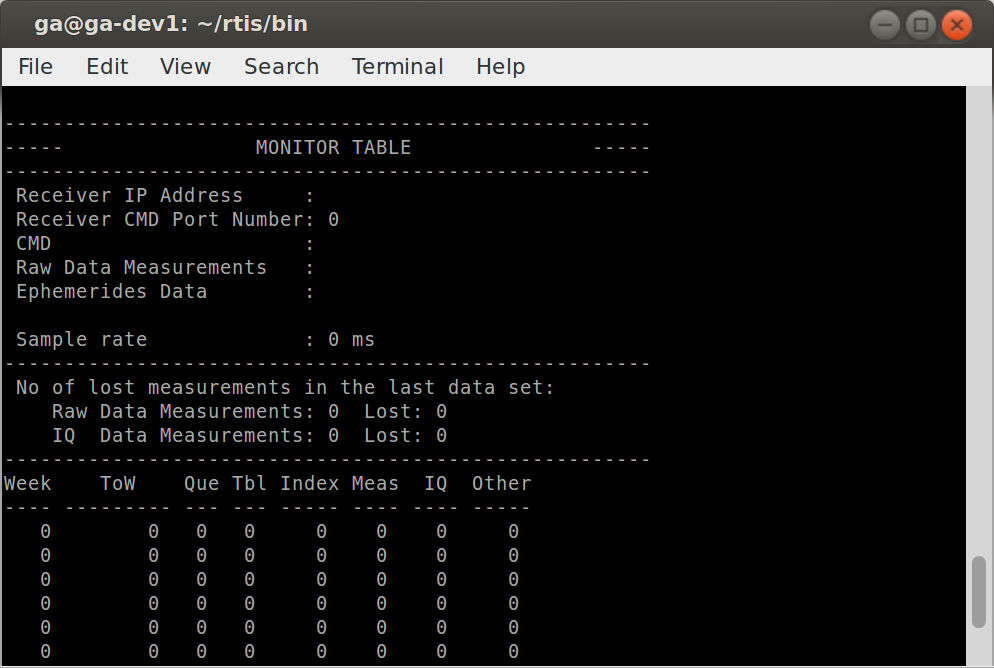
\includegraphics[width=0.5\textwidth]{rtis_mon}
	\caption{Monitoring table as seen with rtis\_mon}
\end{figure}

Although this method works, a few problems arise.
\begin{itemize}
	\item Only one type of information can be displayed at once. It is obviously not possible to display several tables at the same time on a terminal, but opening several terminals and launching several instances of \textit{rtis\_mon} can also pose problems. They will try to access, maintain opened and read from the same shared memory, which is not possible within the RTIS software. \\
	\item The process of connecting to the distant RTIS station via SSH is not intuitive, and requires the user to have a list of the IP addresses of all the remote stations, to look through it to find the one he wants, and then to enter the command in a terminal. This does not allow to quickly browse through all stations or to easily switch between two of them.
	\item Modifying the configuration file of the distant station requires the user to navigate through the file system to find it, and then to edit or replace it. The edition can be done manually, but a FTP connection has to be made in order to send a new file.
	\item The update frequency cannot be chosen by the user. Though it is not a big issue, it can be annoying for the list of active processes for example, which is not going to change a lot, and certainly not every second.
\end{itemize}


%-------------------------------------------------------------------------------

\section{What needs to be done: goals and expected functionalities}

The making of a new GUI obviously aims at solving the aforementioned problems. It should be a web application, preferably a light client. The new GUI should allow the user to quickly see the status of every station, to connect to any of them, and to see any of the monitoring table (corresponding to the \textit{-mon} option in \textit{rtis\_mon}), the list of active processes (\textit{-proc}), or the error messages\footnote{The \textit{error message} denomination encompasses all of the status messages returned by the applications within the RTIS system. The denomination can be misleading, since this also includes success messages.} returned by the software, to reboot the whole RTIS software, or to change its configuration file. In the following, we will refer to the monitoring table as MON, the list of active processes as PROC, and the error messages as ERR.

\subsection{Visualising data}

It should be possible to see any combination of MON, PROC and ERR simultaneously, and to have independent user-defined refresh frequency on each of them. For example, one should be able to choose to see both MON, refreshed every 2 seconds, PROC, refreshed every 3 minutes, and no error message. The "real-time" factor is not very important, as the data will not be subject to high-frequency changes. A delay of a few seconds is acceptable.

Displaying ERR should work differently than for PROC and MON: there will be no refresh frequency for it, and messages will always be displayed as soon as they are sent by the RTIS software. It should be possible, however, to filter them by their severity. Indeed, every error message within the RTIS software has a severity level. Ranked by order of magnitude, the possible levels are: \begin{enumerate*}
  \item Fatal
  \item Error
  \item Warning
  \item Info
\end{enumerate*}
There are also two special unranked levels, Debug and Notice. The user should be able to select a severity level between 0 and 4, and to receive all error messages with a severity lower or equal to the selected level. Choosing the level corresponding to Error, for example, should make visible every message with a severity of Error or Fatal. The user should additionally be able to choose whether he wants any of Debug or Notice messages, regardless of the "main" severity filter he chose.

\subsection{Modifying the RTIS behaviour}

The GUI should not only be able to observe what the RTIS software does, but also to act on it in some ways: it should be possible to change the RTIS configuration file, and to reboot the whole RTIS software.

There are no specification on how modifying the configuration file should be handled. However, a new feature to add is a history of the previous configuration files. It should be possible to retrieve a previous configuration file, and to revert back to it. It should be noted that a change in the configuration file will not take effect until the RTIS is rebooted. It is thus possible to change the configuration file several times in a row without actually changing anything, just to store the configuration files in the history for later. Again, there is no specification on how the storage should be done.

\begin{figure}[!ht]
	\begin{center}
		\begin{tikzpicture}
		\begin{umlsystem}[x=4, fill=red!10]{The Graphical User Interface}
		\umlusecase[y=0, width=2cm]{See state of every station}
		\umlusecase[y=-4, width=2cm]{Connect to a station}
		\umlusecase[x=4, y=-1, width=2cm]{Visualise data}
		\umlusecase[x=4, y=-3, width=2cm]{Load config file}
		\umlusecase[x=4, y=-5, width=2cm]{Send config file}
		\umlusecase[x=4, y=-7, width=2cm]{Reboot}
		\end{umlsystem}
		
		\umlactor[y=-2]{user}
		
		\umlassoc{user}{usecase-1}
		\umlassoc{user}{usecase-2}
		\umlextend{usecase-2}{usecase-3}
		\umlextend{usecase-2}{usecase-4}
		\umlextend{usecase-2}{usecase-5}
		\umlextend{usecase-2}{usecase-6}
		\end{tikzpicture}
	\end{center}
	\caption{Use-case diagram of the GUI}
\end{figure}

\subsection{The problem of the bandwidth}

The stations of the RTIS network are scattered all across continental Norway, some are in Svalbard and there is even one in Iceland. All of these stations are located close to inhabited locations and benefit from good and reliable connections to the internet.

\begin{figure}[!ht]
	\centering
	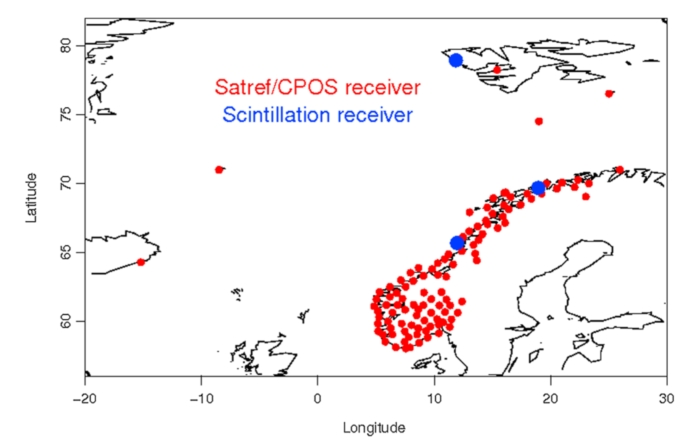
\includegraphics[width=0.5\textwidth]{RtisMap}
	\caption{Map of the stations involved in the RTIS network.}
\end{figure}

But some stations have been placed in extremely remote locations, like Bjørnøya (\textit{Bear Island} in Norwegian), which is not linked to any other place by submarine internet cables, and whose entire internet traffic transits through satellite connections. Due to the costs of bandwidth using these communications, the available bandwidth is very low, and due to to the island being more than 74\degre North, even the satellite connection is unreliable and subject to unpredictable interruptions. 

\begin{figure}[!ht]
	\centering
	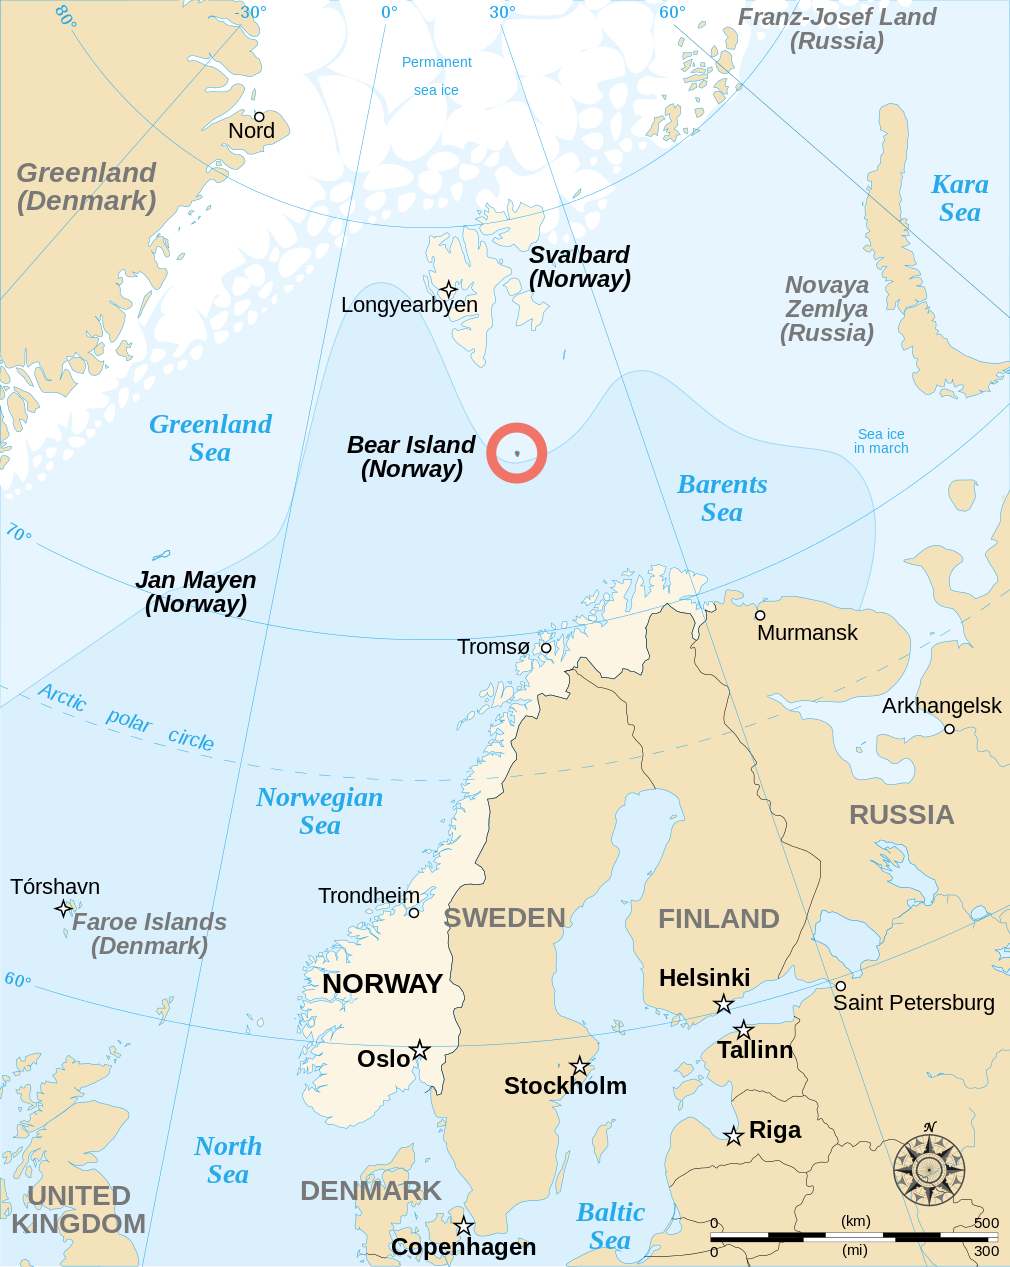
\includegraphics[width=0.5\textwidth]{bearIsland}
	\caption{Location of Bjørnøya © Sémhur, Wikimedia Commons}
\end{figure}

Moreover, there already is data transiting through this connection: the actual observation data that is sent to a calculation centre. One of the requirements for the new RTIS GUI was thus to minimise the amount of data sent or received, to be sure that every message could be received on time, and would not conflict with the observation data for the broadband access. The number of exchanges and/or the size of messages exchanged between the GUI and the stations should be as small as possible.

It was also demanded that the remote RTIS station would somehow detect if the connection with the GUI had been broken, and stop sending data through a broken pipe. The user should still be able to cleanly disconnect from the station to stop receiving data from it, but in the event of a breakage of a connection, it should also be able to detect it and not indefinitely continue sending data while waiting for a disconnection signal from the GUI.

\subsection{Miscellaneous}
The website should be able to be visited on any kind of support, with any kind of OS: Linux and Windows computers, Android and iOS phones... This has technical implications and implies to check compatibility when choosing of technologies, and also influence the design of the web page, which should be responsive and adapt to mobile devices with a smaller screen.

About the languages to code the website in, the choice is limited to PHP or Java. Although some other  technologies might be tempting, like Node.js for the real-time display, all the maintenance of the my work is going to be done by the team behind RTIS, and they logically chose to limit the technologies involved to the ones they were familiar with.

It is not required to have any login system, nor to be able to deal with simultaneous users on the GUI. It is only meant for an internal use, with restricted access. Anyone able to access the website is able to do all the interface allows to do. I am not aware of the inner workings of the internal network in Kartverket, and am only expected to have the product working on my development server. They will deal with the deployment.

%-------------------------------------------------------------------------------
\evenchapter[The proposed solution]{The proposed architecture}
%-------------------------------------------------------------------------------
\section{General considerations}

The solution I have come up with is a light client: since there are no calculations nor any resource-consuming operation that is going to be needed, everything will be done on the web server without any risk of overloading it.

The website is coded in PHP, because it is a language I and the RTIS team are familiar with. The main other option was Java, which I do not really know nor like. Moreover, while environments like J2EE could be useful for bigger projects, this relatively simple interface does not require such a complex technology.
As the RTIS program is written in C and includes some low level libraries for communications, all of the code behind the interface used to communicate with the RTIS system will be written in C as well.

Also, while the GUI can ask for the RTIS software to send data, it cannot directly fetch it: some modules have to be added directly in the RTIS software, in the distant stations, to be able to communicate with them.

\section{Architecture}
\subsection{Global overview}

The general architecture of my solution is presented in figure 2.1.

\begin{figure}[!ht]
	\centering
	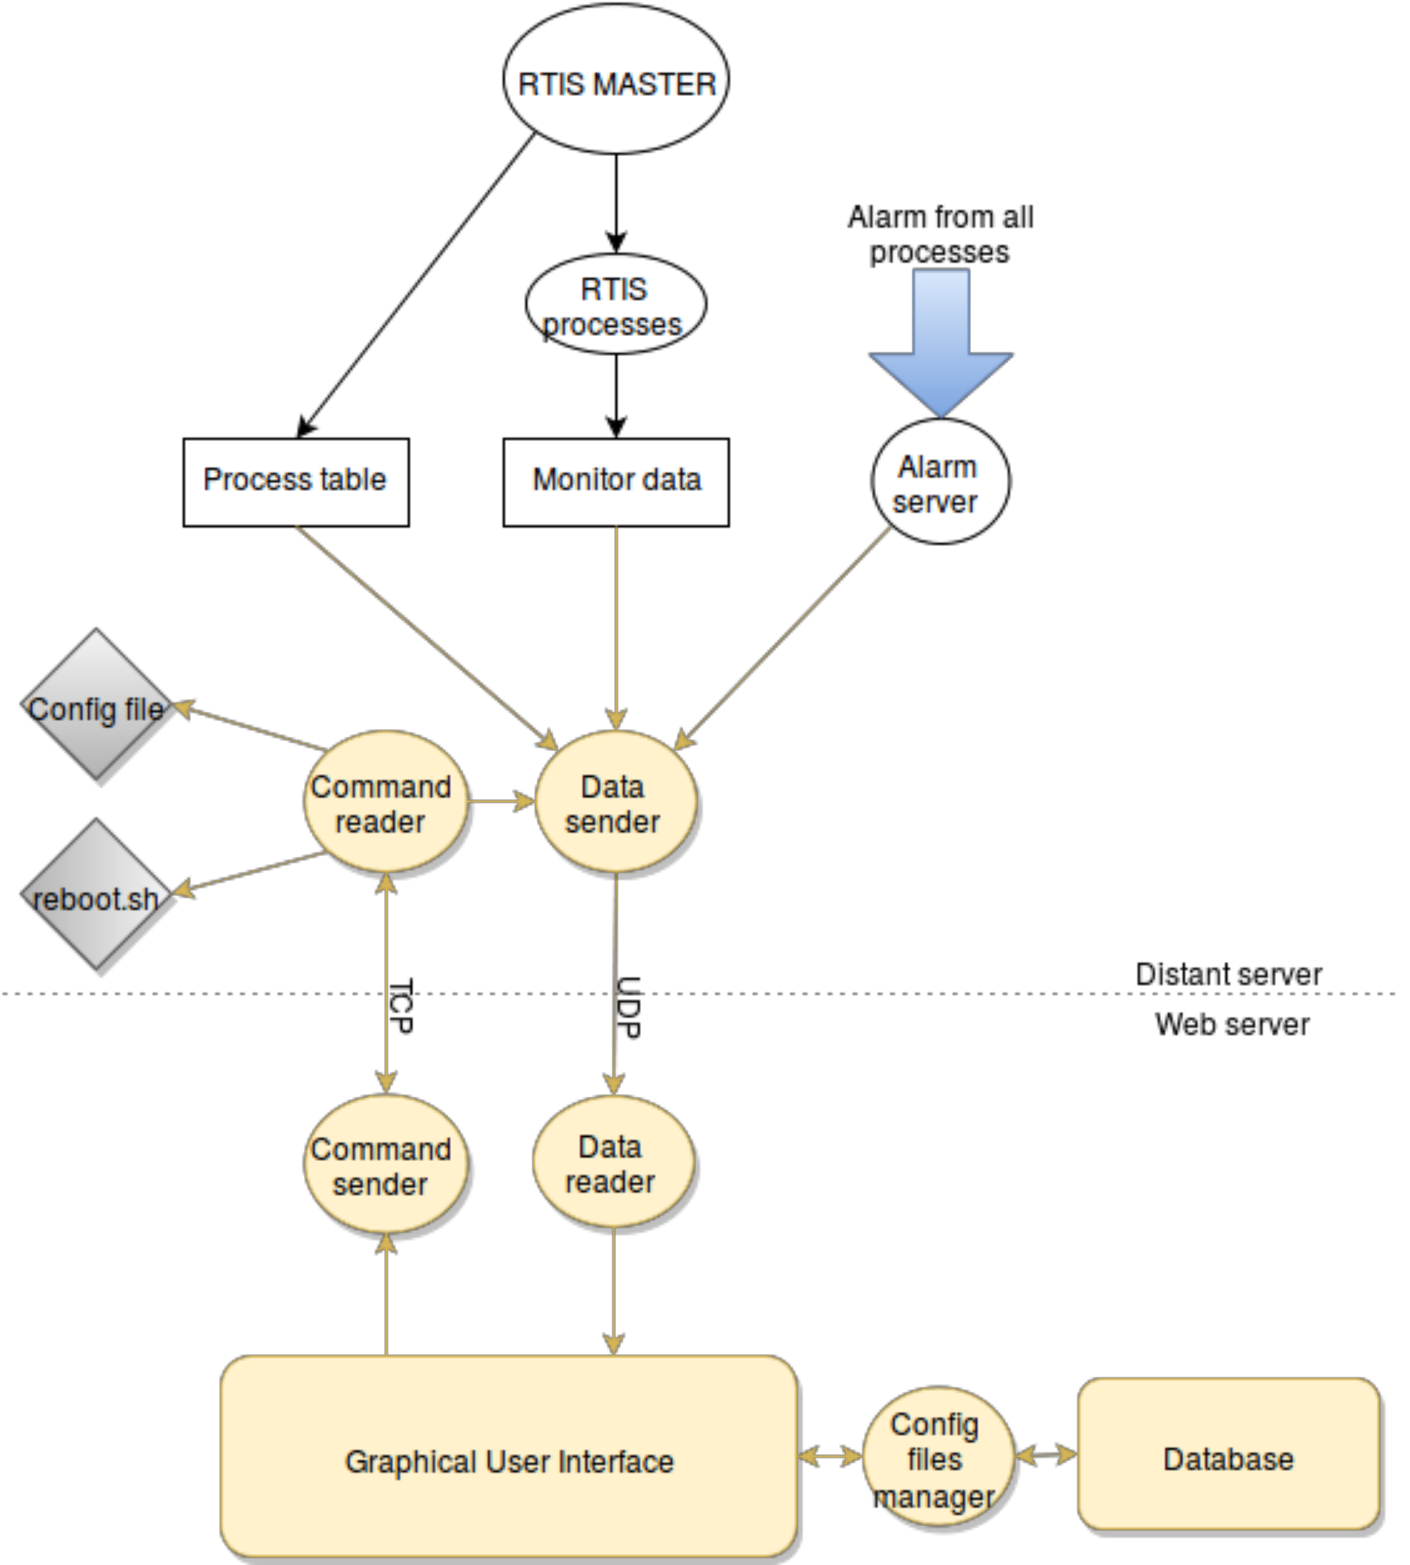
\includegraphics[width=0.8\textwidth]{global_flowchart}
	\caption{General organisation of the solution, working document}
\end{figure}

In white, we have a schematization of the existing RTIS software, which will be detailed, and in yellow are a simplified version of the modules and programs I should develop.

\subsubsection{A brief overview of the RTIS software}

First, let us go through the existing RTIS software to better understand how I will interact with it. Right on top, we have the GNSS receiver, whose role is obviously to collect data. This data is stored into one of the two data buffers, while the other one is being processed by the RTIS software. Every buffer contains one minute of observations, which implies that RTIS can take up to one minute to process one minute of data. If it takes longer, the buffers are swapped anyway, the remaining data is erased by new observations, and is thus lost. This can happen in period of strong ionospheric activity, hence the need for the modules I add to take as few resources as possible.

Just underneath the GNSS receiver, we have the Controller. It is responsible for managing all the modules that do the processing, ensuring that they are all up and running, and relaunching them if necessary. To reboot the whole RTIS system, one only needs to reboot the Controller.

We then have a lot of independent processes that process data, store their intermediate or final results in a shared memory, and then send the results to a control center in Kartverket. Now, we will only be interested in some parts of the shared memory that we want to read. We do not need to know any more about the inner workings of the software or its data.

\subsubsection{The general idea behind the architecture}

We will here refer to the web server that hosts the GUI as "the server" and to the distant RTIS installation as "the client".
The architecture is pretty straightforward: the GUI can send commands to the client via the \textit{Command Sender}, which are then read on the client by a dedicated \textit{Command Reader}. Depending on the message, the \textit{Command Sender} will either modify parameters of the \textit{Command Reader}, update the configuration file on the client, or launch a bash script to reboot the system. The \textit{Data Sender} reads data from the RTIS shared memory according to what the \textit{Command Reader} demands, and sends it back to the GUI, which then reads and displays it.

There are two types of connections that link the server to the client: the server sends its request with the TCP protocol, while the client sends its data using UDP. The reason for that is that the TCP protocol offers a very reliable connection: whenever a message is sent through a TCP stream, it is almost certain that it will be received on the other side. The receiver has to send a confirmation of the reception of the message, and if the sender does not receive the confirmation, it will send the message again. As we want to be sure that our commands have been sent, this is the solution to use here.
The UDP protocol, on the other hand, does not perform any check, nor needs the receiver to actually be connected. It just sends data and hopes that it will be received on the over side. Although obviously less reliable than TCP, it is also much faster for real-time applications: if the message has not been received, there is no point in trying to re-send it as it is already obsolete, and we need to send new messages with the new data instead. What matters here is sending information quickly, and if some of it is lost, it is not a major problem.

About the history of configuration files, now. To limit the use of bandwidth, whenever the user wants to view the history of the configuration files for a station, or even the current configuration file, it is not efficient to fetch it from the client: even though these files only weigh 2kB, this would result in unneeded bandwidth usage.
A database has thus to be created on the server, where configuration files are duplicated whenever they are sent to the client. This way, we are ensured to always have all of the configuration files handy without any need for costly data transfer.


\subsection{In-depth descriptions of the modules}

\begin{figure}[!ht]
	\centering
	\includegraphics[width=\textwidth]{detailed_flowchart2}
	\caption{Detailed organisation of the modules, working document}
\end{figure}

First of all, all communications between client and server are made via SATREF messages. These messages are a Kartverket standard, can convey any kind of information, and aim to be as small as possible by converting all the values it contains in binary format. Kartverket has developed high-level C libraries to write and read these messages.

\subsubsection{Command senders}

Commands senders are a combination of PHP and C scripts. Their role is, as their name suggests, to convert user input from the GUI into a command, and to send it. There is one command sender per type of command that can be sent: fetch ERR, fetch MON, fetch PROC, send configuration file, reboot. The command reader will make the difference between all of these types of messages based on their type, an integer placed into the header message. Thus, most of the messages going from the server to the client do not even need a body: they will just consist of a header whose only meaningful information will be the message type, the only exception to that being for configuration file updating.
If the user has entered in the interface that he wants to see MON, refreshed every 7 seconds, the PHP script will just call, every 7 seconds, the C script whose job is just to create and send one specific message. And every 7 seconds, a message of type "MON" will be sent to the client to notify it that it needs to immediately send MON data. It works the same way with PROC.

The "Reboot" command consists of a single message, exactly like for MON \& PROC, though sent only once. 

For ERR, however, one cannot simply choose the frequency of the updates: if ERR is enabled, messages will be sent as soon as they are emitted by the client. The technique of "sending a message per update" used for MON and PROC cannot be used anymore. Here, only one message will be sent every two minutes (this step can be changed). When received, the \textit{Data Sender} will send messages for the next two minutes. While not optimal, this method, like the one used for PROC \& MON, fulfil the requirements: the messages sent from the server are extremely small in size, and if the server-client connection is broken, the \textit{Data Sender} will stop sending messages.

Finally, when sending a configuration file, the whole file is parsed, all of its values are extracted before being put, one after the other, into the SATREF message. The size of the message is greatly reduced compared to the file's one: only the values are taken into account, while the file has a lot of text that does not change from one file to the other and is thus useless to send. An example of a configuration file is given on Annex A.

All of these messages need to be acknowledged by the receiver, who should send an empty SATREF message back at the sender. Only then would the command sender know that its command has been received and obeyed to. Should this confirmation message not be received, the command will be sent again, until a certain period of time is elapsed. If no answer is received then, an error notification is sent to the GUI, that will display it. This whole process of confirming the messages is arguably redundant with the very idea of choosing a TCP connection, but we do not only want to be sure that the message has been received, we also need to be sure that it has been processed.

\subsubsection{Command reader \& data sender}

The command reader consists of only one program, constantly running and listening for messages. The way things are done here are that the TCP server that listens to messages is set in "blocked" mode. Concretely, "non-blocked" would have meant having an infinite loop running at full speed and checking at every iteration for messages to read, thus asking a lot from the CPU, while "blocked" just puts the program to sleep and wakes it up whenever a message comes, which is a lot more efficient.

Once a message is received, it adjusts its behaviour depending on the nature of the message, indicated by the "message type" contained in the header. If the message is asking for PROC or MON, it will read it from the shared memory, once, convert it into a SATREF message, send it to the \textit{Data Reader} (via UDP) and send a confirmation to the \textit{Command Sender} (via TCP), before putting itself to sleep once more and waiting for new messages.
A "reboot" message will result in a system call to launch a bash file on the client, that will do the rebooting. As with any kind of received message, a confirmation is then sent to the command sender.
For configuration files, the contents of the message are converted to C variables, a configuration file is written based on these variables, and is moved to erase the old file.

The tricky part here was for the error messages. Indeed, and unlike the other messages, what these commands ask for not is not a "once only" behaviour. A single command asking for ERR means fetching it for the next 2 minutes. If it was left in the same flow of execution as the command reader, that would interrupt its normal behaviour and prevent it from reading any other command from the GUI while the errors are fetched.
Moreover, the method for storing and reading the error messages within the RTIS software is a bit special. They are stored in a ringbuffer, which means that if the messages are not read quickly enough, they will get erased by new ones. To read that, a function exists within the RTIS libraries: once more, it is set to a "blocked" mode, which means that it will read new messages when they come, remove them from the ringbuffer, and go back to sleep immediately after.
To deal with the problem of the infinite loop of waiting for error messages within the infinite loop of waiting for GUI commands, I have resorted to a fork of the \textit{Command Sender} program. I detail the general idea in the following figure.


\begin{figure}[!ht]
	\centering
	\begin{algorithmic}
		\State $hasForked \gets False$
		\While{True}
			\State $message \gets listenMessages(blocked=True)$
			
			\If{$message.Type == errType$}
				\If{$!hasForked$}	
					\State $hasForked sgets true$
					\State $pid \gets fork()$
				\EndIf
				\If{$pid == 0$}
					\While{True}
						\State DO STUFF
					\EndWhile
				\EndIf
			\EndIf
		\EndWhile	
				
				
	\end{algorithmic}
	\caption{Explanation of the algorithm}
\end{figure}


\subsubsection{Data reader}

%-------------------------------------------------------------------------------
\clearpage
\section{The GUI}
\subsection{Receiving data: trying to be intuitive}

bootstrap
responsive


%-------------------------------------------------------------------------------
\newpage
\subsection{Sending files}

Both by input fields or by sending file (not asked for). Check for correct file. Check for malicious input. Connection to db. Loading file prefills the fields (not asked for). Possibility to add a name to file to find it more easily (not asked for). Possibility to delete file from db (naf). 
%-------------------------------------------------------------------------------
\newevenpage
\chapter*{Conclusion}
  \addcontentsline{toc}{part}{Conclusion}
  \vspace{1.5cm}

\newevenpage
\begin{appendices} 
\label{beginappendices}

\annexe[Example of a RTIS configuration file]{Example of a RTIS configuration file}
\label{configfile}

\lstinputlisting[language=Lisp]{resources/rtis_config.cfg}

\end{appendices}


\end{document}